\documentclass{standalone}
\usepackage{tikz}
\usetikzlibrary{positioning}

\begin{document}
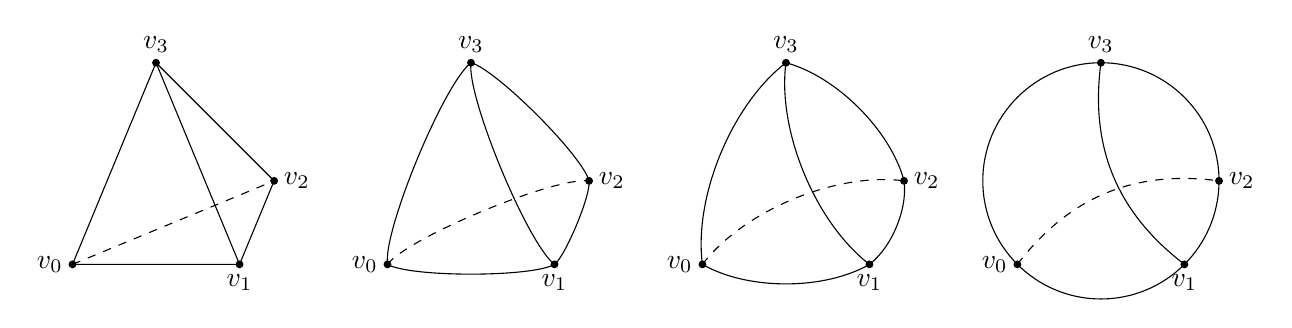
\begin{tikzpicture}
  \begin{scope}[shape=coordinate, name prefix=1-]
    \node (top) at (90:1.5){};
    \node (bottom) at (-45:1.5){};
    \node (left) at (-135:1.5){};
    \node (right) at (0:1.5){};
  \end{scope}
  
  \fill (1-top) circle (0.05) node[above]{$ v_3 $}; 
  \fill (1-bottom) circle (0.05) node[below]{$ v_1 $}; 
  \fill (1-right) circle (0.05) node[right]{$ v_2 $}; 
  \fill (1-left) circle (0.05) node[left]{$ v_0 $}; 

  \draw (1-bottom) to (1-right) to (1-top) to (1-left) to cycle;
  \draw (1-bottom) to (1-top);
  \draw[dashed] (1-left) to (1-right);

  \begin{scope}[xshift=4cm]
    \begin{scope}[shape=coordinate, name prefix=2-]
      \node[right = 4cm of 1-top] (top){};
      \node[right = 4cm of 1-bottom] (bottom){};
      \node[right = 4cm of 1-right] (right){};
      \node[right = 4cm of 1-left] (left){};
    \end{scope}

    \fill (2-top) circle (0.05) node[above]{$ v_3 $}; 
    \fill (2-bottom) circle (0.05) node[below]{$ v_1 $}; 
    \fill (2-right) circle (0.05) node[right]{$ v_2 $}; 
    \fill (2-left) circle (0.05) node[left]{$ v_0 $}; 

    \draw[bend right, looseness=0.4] (2-bottom) to (2-right) to (2-top) to
      (2-left) to cycle;
    \draw[bend left, looseness=0.4] (2-bottom) to (2-top);
    \draw[dashed, bend left, looseness=0.4] (2-left) to (2-right);
  \end{scope}
  

  \begin{scope}[xshift=8cm]
    \begin{scope}[shape=coordinate, name prefix=3-]
      \node[right = 8cm of 1-top] (top){};
      \node[right = 8cm of 1-bottom] (bottom){};
      \node[right = 8cm of 1-right] (right){};
      \node[right = 8cm of 1-left] (left){};
    \end{scope}

    \fill (3-top) circle (0.05) node[above]{$ v_3 $}; 
    \fill (3-bottom) circle (0.05) node[below]{$ v_1 $}; 
    \fill (3-right) circle (0.05) node[right]{$ v_2 $}; 
    \fill (3-left) circle (0.05) node[left]{$ v_0 $}; 

    \draw[bend right, looseness=0.8] (3-bottom) to (3-right) to (3-top) to
      (3-left) to cycle;
    \draw[bend left, looseness=0.8] (3-bottom) to (3-top);
    \draw[dashed, bend left, looseness=0.8] (3-left) to (3-right);
  \end{scope}

  \begin{scope}[xshift=12cm]
    \begin{scope}[shape=coordinate, name prefix=4-]
      \node[right = 12cm of 1-top] (top){};
      \node[right = 12cm of 1-bottom] (bottom){};
      \node[right = 12cm of 1-right] (right){};
      \node[right = 12cm of 1-left] (left){};
    \end{scope}

    \fill (4-top) circle (0.05) node[above]{$ v_3 $}; 
    \fill (4-bottom) circle (0.05) node[below]{$ v_1 $}; 
    \fill (4-right) circle (0.05) node[right]{$ v_2 $}; 
    \fill (4-left) circle (0.05) node[left]{$ v_0 $}; 

    \draw (0,0) circle (1.5);
    \draw[bend left, looseness=1] (4-bottom) to (4-top);
    \draw[dashed, bend left, looseness=1] (4-left) to (4-right);
  \end{scope}
\end{tikzpicture}
\end{document}
